\documentclass[11pt]{article}

\usepackage{amsmath,amssymb}
\usepackage{a4wide}
\usepackage{graphicx}
\usepackage{tikz}
\usepackage{algorithm}
\usepackage{algorithmic}
\usepackage{parskip}

\newcommand{\maxsize}[1]{\begin{quotation} {\sl \noindent Maximum size: #1.} \end{quotation}}

\newcommand{\crp}[1]{\begin{quotation} {\sl \noindent For the curve- and network-reconstruction problem: #1} \end{quotation}}

\newcommand{\example}[1]{\begin{quotation} {\sl \noindent Example: #1} \end{quotation}}

%%
% Theorem-Like Environments
%
\newtheorem{defin}{Definition}
  \newenvironment{mydefinition}{\begin{defin} \sl}{\end{defin}}
\newtheorem{theo}[defin]{Theorem}
  \newenvironment{mytheorem}{\begin{theo} \sl}{\end{theo}}
\newtheorem{lem}[defin]{Lemma}
  \newenvironment{lemma}{\begin{lem} \sl}{\end{lem}}
\newtheorem{coro}[defin]{Corollary}
  \newenvironment{corollary}{\begin{coro} \sl}{\end{coro}}
\newtheorem{obse}[defin]{Observation}
  \newenvironment{observation}{\begin{obse} \sl}{\end{obse}}

\newenvironment{proof}{\emph{Proof.}}{\hfill $\Box$ \medskip\\}

% TODO(robwu): Choose a more descriptive title
\title{2D curve and network reconstruction}
\author{
A. van den Boogaart \and
W. Brouwer \and
C. Mens \and
M. Muijsers \and
R. Wu
}
\date{\today}

\begin{document}

\newpage

\maketitle

\begin{abstract}
We present three algorithms that connect all nodes in an unorganised set in the 2D plane in an aesthetically pleasing manner. 
The first algorithm will reconstruct a set of nodes into a single curve, such that no lines intersect. 
The second algorithm will create multiple curves from the set of nodes, also in such a way that no lines intersect. 
The third and final algorithm will attempt to create a road network from the nodes, and can add additional nodes when intersections occur.

\end{abstract}

\section{Introduction}
\label{se:introduction}
The to be presented algorithms will solve the problem of reconstructing curves for a given set of points in the 2D plane. This problem has three slightly different forms: The first two require the reconstruction of a set of points into curves, in the first case there is only one curve, whereas in the second case there are multiple. The third part of the problem requires reconstructing to a road network.

The first two curve reconstruction algorithms are subject to some constraints: Curve segments should not intersect each other and all points in the input must be used in the curve.

The goal of the road network algorithm is to create a reasonable representation of the road network, such that a person would agree with the representation that the algorithm gives. This algorithm could be used to create a road map after data has been collected using the GPS locations of cars.

As with the other algorithms, there are some constraints: All points need to have at least one possible path to every other point and lines cannot intersect one another. However, unlike the other problems, points can be added to alleviate intersecting lines.

All nodes are points in a 2D plane, represented by floating point numbers ranging from 0 to 1. These nodes are not calculated by the algorithm, but determined in advance. In practice, these datasets can be created by laser scanners, or in the case of the network, by following roads and giving the location at some interval.

There are multiple known solutions to these problems. One of these is 'The Crust Algorithm' \cite{crust}, which first creates a Voronoi diagram, then uses Delaunay triangulation between the Voronoi diagram and the Voronoi vertices. The Crust Algorithm solves the first problem that is described above, but needs additional work to determine the multiple curve problem.

Delaunay triangulation could also be used to create a relatively small set of edges for the third problem, after which a rectilinear spanning graph or straight lines can be determined between points. The Crust algorithm is however fairly complicated, and we do not think it is viable to recreate this within the given time.

For the single curve reconstruction problem, we have also looked at the convex hull. A convex hull will create segments between all the outermost points, such that no unconnected point is outside of the enclosed area. Like putting a rubber band around all the points. This can be very useful for connecting the outermost edges, but it is not as useful for inner edges.

A very useful subgraph that we looked at is the rectilinear spanning tree. This is a minimum spanning tree based on rectilinear distance, which is very much like manhattan distance, and is useful because it already has all the properties that the network reconstruction requires; It connects the points in such a way that there is a path from every node to every other node and there are no intersecting lines.

To solve the single curve reconstruction problem, we have chosen for a spider-type algorithm, which will go from point to point and then determines the next best point to go to.

The multiple curve and road network reconstruction problems are solved using a minimum spanning tree. In multiple curve construction problem, the graph is completed using an adjacency matrix and another supporting data structure. The road network problem uses a particular kind of spanning trees, namely rectilinear minimum spanning tree to get an initial solution the problem. After reconstructing this tree, we try to find straight lines and connect those, since a spanning tree will not create cycles.

\newpage
\section{The algorithms}
\label{se:algorithms}

\subsection{Single curve reconstruction}
To solve reconstruction of a single curve, we took an intuitive approach. After analyzing our own train of though when solving our own test cases, it was clear that our brains were trying to start somewhere on the curve, and following the curve along, making sure no points got forgotten in time.

We have attempted to utilize a similar method. We implemented a 'spider'-type algorithm that mainly depends on three important steps:
\begin{itemize}
\item Choose a position for the spider to start
\item Let the spider decide where it wants to go next, based on factors
\item Let the spider go there and have it connect the two nodes
\item Go on until the beginning has been reached
\end{itemize}

This interpretation soon raises the question "So how does it make sure no points are forgotten?".
When two curves come really close to each other, the spider might feel like a node in the other curve is the best place to go, thus probably completely invalidating the rest of the run.

A simple solution for this would be to see at the end whether the found curve is a valid curve, and to rewind to a point where the algorithm likely made the wrong choice.

\subsubsection{Naive implementation} 

Attempting to implement this solution, which we will name the Spider algorithm from here on, lead to disappointing results. Analyzing the informal description already soon tells you the running time of a naive implementation will definitely not be $O(n!)$, and this is what we found after implementation.

Without the recursive strategy of looking back and trying to find a point where a mistake was made, the algorithm performs quite fine and finds a nice line (sometimes intersecting). With the recursive strategy, the algorithm takes too long to run on any amount of points larger than 100, where the points are considerably random.

These observations of the naive implementation lead us to create a more clever version of the Spider algorithm, that supported:
\begin{itemize}
\item Smart choice of a first position
\item Smart choice of next node depending on all available factors
\item A manageable way of remembering possibly valid choices and re-evaluating those choices if necessary
\item A solid way of identifying mistakes
\end{itemize}


\subsubsection{Choice of first position} 

The first position of the spider will be chosen by picking the most boundary-like point. The most boundary-like point is the point, which has the largest continuous angular interval where no other points lie. So, if the spider were standing on the most boundary-like point, it could look around that whole angular interval and see no points.

The first segments are then chosen by taking the two nearest nodes, and since there are then 3 possibilities to form 2 segments (we do not want to form a triangle unless there are only 3 points, of course) we simply take each of them and process each of them, and see which one fails the least.

\subsubsection{Choice of next node} 

If the spider is standing at a certain node, it looks back at the nodes it came from, and decides on the expected angle and distance to the next node. The expected angle is a continued value of a linear formula with the previous 2 angles as anchor points, and the expected distance is a continued value of a linear formula with the previous 2 distances as anchor points. In simpler terms: the change in angle and distance between the two last traversed segments is expected to be closely the angle and distance between the last traversed segment and the next to traverse. If the last traversed distances are 4 and 6, the expected next distance will be 8.

The nodes are then sorted and stored by their 'likelihood' to be the best successor. Their likelihood is defined as the result of a (chooseable and possibly adaptive) formula that determines how close the observed angle and distance to a point being evaluated is to the expected angle and distance to observe.

The node with the best likelihood is then selected to be the successor and the spider moves to that node. (Whether a smaller or greater likelihood means more likely can depend on implementation if it is mathematically easier. We will not speak about the data representation of likelihood except for the fact that we chose to use a float value decreasing if more likely.)

The formula that we used for the likelihood is the sum of squares of the following values: the ratio of distance to the expected distance (if smaller than 1, this value is taken to the power -1), and the absolute difference in angle to the expected angle (in fraction of pi).

\subsubsection{Remembering possibly valid choices} 

For the whole path taken, per node it is stored what the though process at that point was (a 'viewpoint'): a sorted list of possible nodes to travel to, and their likelihood. When a mistake is made, we can simply look at the difference of the current likelihood to the next likelihood per viewpoint, and choose the one which is most likely incorrect to change.

\subsubsection{Identifying mistakes} 

To identify mistakes, we used the following criteria:
\begin{itemize}
\item The node the spider wants to go is VERY likely (a certain factor of difference to the next likelihood) but requires an intersection
\item The last segment would create an intersection, and it not too long to be removed
\item Not all nodes have been taken into account when the last node is reached
\end{itemize}


\subsubsection{Open or closed} 

Finally, we would like to spend a word on the detection of whether a curve is open or closed. We first decided that whether a curve is open or closed depends on the factor between the longest segment length and the one-to-longest segment length: if this is large enough, the curve is probably open and we should remove the longest segment.

However, the distances between nodes may vary greatly in parts of the curve. Therefore, we decided on a slightly different alternative: whether a curve is open or closed depends on whether there is a segment, for which the factor between its own length and the lengths of its adjacent segments is higher than a certain number. If so, the segment with such highest factor should be removed.

\subsection{Multiple curve reconstruction}

\subsubsection{Outline}
Our multiple curve reconstruction algorithm is based on findings after an evaluation of how humans find curves in a set of points. By consciously observing ourselves while connecting nodes, we have found that the most important factors in determining whether or not to connect a point to another point are 1) the proximity of other points and 2) line segment patterns in the graph constructed so far.

In order to develop an algorithm that uses these concepts, the most important primitives for building the algorithm have to be identified. This step is important, because an algorithm that yields a perfect solution is useless when it takes ages to calculate the result. The two important factors from the previous paragraph resulted in the following supporting primitives:

\begin{itemize}
\item Adjacency matrix - By calculating an adjacency matrix in advance, the algorithm can find nearby points in constant time.
\item \textsc{ConnectedNodes} - A data structure that provides information about the connected nodes in a graph. In particular, it answers the following questions:
\begin{itemize}
\item Given a line segment, does it intersect the graph?
\item Given a node, which segments are connected to it?
\item Which nodes in the graph are connected to at most one other node?
\end{itemize}
\end{itemize}

The actual algorithm starts with calculating a minimum spanning tree for all input nodes. Thereafter, nodes that are not yet connected with two other nodes are located and connected to the most appropriate neighbor. These neighbors are found with help of the previously mentioned primitives. Finally, clusters of coherent nodes are separated from other nodes. The details for this algorithm are elaborated in the next section.

\subsubsection{Description}
The algorithm takes a set of $n$ Nodes (with an X and Y coordinate) as input, and yields a set of Segments (a data type with two (x,y) coordinates denoting its endpoints).

At first, an Adjacency matrix is constructed from the set of nodes. This takes $O(n^2)$ time. This matrix is stored in a hashmap that maps nodes to an array of node-distance tuples. This list is sorted in ascending order by the distance between the node and key. Because there are $n$ lists to be sorted, and a comparison-based sorting algorithm is mandatory, the running time of this step is $O(n^2 \log(n))$. After this expensive set-up, queries such as finding the Xth closest node to a node can be answered in constant time.

\textsc{ConnectedNodes} is responsible for maintaining the information about the segments between the nodes. A mapping from nodes to neighbors can be maintained and accessed in constant time: Whenever a new segment is added to the graph, also add the segment to the sets of neighbors of both endpoints.

To know whether a segment intersects the graph, a segment must be compared to all $k$ other segments. When there is no intersection, this algorithm takes $O(k)$ time. This is an acceptable method if the algorithm uses this operation about $k \log(k)$ times, because the final graph will have approximately as many segments as nodes.\\
If it turns out that this is too slow, then it can be optimized by reducing the query space: If every segment was wrapped in a rectangle, then it is obvious that there are segments that will never intersect some other segment. This concept can be implemented by maintaining four sorted lists of the coordinates of the two opposite corners in the rectangle (minX, minY, maxX, maxY). A disadvantage is that adding or removing segments will no longer take constant time, but $O(\log(k))$ time, because the location of the segment has to be identified using binary search. At the same time, the worst case running time is still $O(log(k))$, but on average it will have a much smaller constant, because the boundaries of the query space can be found using binary search. For a large set of nodes, the rectangles are expected to be small, because the segments will probably connect to a near node rather than a node at the other side of the graph.

After setting up the basic primitives, a MST is calculated, e.g. by calculating the permutation of all segments between all nodes followed by running Kruskal's algorithm \cite{k-osssgtsp-56} on the result. This takes $O(n^2\log(n))$ time and yields $n$ segments. These $n$ Segments are added to \textsc{ConnectedNodes}.

After constructing the adjacency matrix and \textsc{ConnectedNodes} with the MST, follow the following steps:

\begin{enumerate}
\item Find all segments with only one segment and connect it to its closest neighbor (this takes $O(log(n))$ time).

\item Find all cycles in the graph, e.g. using Depth-First-Search.

\item\label{algo:rob-step-three} Find all segments that are connected to a node with three or more segments, and remove these from the graph, provided that it does not break a cycle.

\item Find all overlapping cycles and try to split the cycles, by trying to disconnect the segments past the common path (the set of consecutive segments that the cycles have in common) and reconnecting the two nodes with degree 1. If this step fails to split the cycle, revert the attempt and continue with the next overlapping cycle until all overlapping cycles have been processed.

\end{enumerate}

This algorithm might give even better results if the distance between nodes is accounted for at step \ref{algo:rob-step-three}

\subsection{Network Algorithm}
\subsubsection{Background definitions}
\begin{itemize}
  \item $\mathbb{R}^2$ is the two dimensional Euclidian space.
  \item $P$ is the given set of points in $\mathbb{R}^2$
  \item $L_1$ distance is the distance between two points in taxicab geometry.
  \item Rectilinear minimum spanning tree $RMST$is the tree spanning all points in $P$ such that the sum of its edge $L_1$ distances is the minimum.
  \item $RN_{min}$ is a minimum reconstruction of the road network that adds missing straight road segments to the $RMST$.
  \item $RN_{com}$ is a complete reconstruction of the road network in which juctions and roundabouts are connected in a correct way.
\end{itemize}
\subsubsection{Outline}

The algorithm consists of the following steps:
\begin{enumerate}
  \item Given a set $V$ of points in $\mathbb{R}^2$ create a graph $G(V,E)$ where $V=P$ and $E=V\times V$.
  \item Compute the $RMST$ of $G$.
  \item Mark points that are only in one segment and find $RN_{min}$.
  \item Find segments with a divergent angle and compute $RN_{com}$.
  \end{enumerate}
  
\subsubsection{Description}
Given the set $V$ of points in $\mathbb{R}^2$ we first generate a graph $G$ in which every point $p\in V$ is connected to every point $q \in V$. Then the algorithms computes the $RMST$, see algorithm \ref{alg:RMSTalg}, using Kruskal's algorithm \cite{k-osssgtsp-56}, for $G$ resulting in a connected graph that gives a good approximation of the road network but some straight road segments may not be connected, see figure \ref{fig:RMST}.

We now find a set of points $S$ for which every $s \in S$ is a endpoint of a road segment, see algorithm \ref{alg:RNminalg}. For these points a edge $e \in E$ is found such that $e=(s,x)$ where $x \in V$. The slope of the edge determines the direction for the road segment for which $s$ is the endpoint. A line $l_1$ perpendicular to the slope is calculated and it is checked whether a nearby point $x \in V$ is below $l_1$ for $e$ with a negative slope or if $x$ is above $l_1$ for $e$ with a positive slope, see figure \ref{fig:RNmin}.

Finally we calculate $RN_{com}$, see algorithm \ref{alg:RNcomalg}. First we find all segments $e \in E$ for which the slope of the following segment $e' \in E$ is divergent. For the segment $e$ we draw a line in the same direction and look for a intersection with a segment $x \in E$, see figure \ref{fig:RNcom}. If the distance between $e$ and $x$ is sufficiently small segment $e'$ is removed from $RN_{min}$ and a new segment from $e$ to $x$ is added to $RN_{com}$.

\begin{figure}
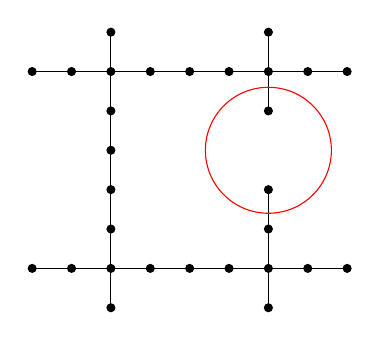
\begin{tikzpicture}
\draw [fill] (7,0.5) circle [radius=0.05];
\draw [fill] (7.5,0.5) circle [radius=0.05];
\draw [fill] (8,0.5) circle [radius=0.05];
\draw [fill] (8.5,0.5) circle [radius=0.05];
\draw [fill] (9,0.5) circle [radius=0.05];
\draw [fill] (9.5,0.5) circle [radius=0.05];
\draw [fill] (10,0.5) circle [radius=0.05];
\draw [fill] (10.5,0.5) circle [radius=0.05];
\draw [fill] (11,0.5) circle [radius=0.05];
\draw [fill] (7,3) circle [radius=0.05];
\draw [fill] (7.5,3) circle [radius=0.05];
\draw [fill] (8,3) circle [radius=0.05];
\draw [fill] (8.5,3) circle [radius=0.05];
\draw [fill] (9,3) circle [radius=0.05];
\draw [fill] (9.5,3) circle [radius=0.05];
\draw [fill] (10,3) circle [radius=0.05];
\draw [fill] (10.5,3) circle [radius=0.05];
\draw [fill] (11,3) circle [radius=0.05];
\draw [fill] (8,0) circle [radius=0.05];
\draw [fill] (8,1) circle [radius=0.05];
\draw [fill] (8,1.5) circle [radius=0.05];
\draw [fill] (8,2) circle [radius=0.05];
\draw [fill] (8,2.5) circle [radius=0.05];
\draw [fill] (8,3.5) circle [radius=0.05];
\draw [fill] (10,0) circle [radius=0.05];
\draw [fill] (10,1) circle [radius=0.05];
\draw [fill] (10,1.5) circle [radius=0.05];
\draw [fill] (10,2.5) circle [radius=0.05];
\draw [fill] (10,3.5) circle [radius=0.05];

\draw (7,0.5) --(11,0.5);
\draw (7,3) --(11,3);
\draw (8,0) --(8,3.5);
\draw (10,0) --(10,1.5);
\draw (10,2.5) --(10,3.5);

\draw [color=red] (10,2) circle[radius=0.8];


\end{tikzpicture}
\caption{$RMST$ for $P$ with a missing road segment indicated by the red circle.}
\label{fig:RMST}
\end{figure}

\begin{figure}
\begin{tikzpicture}
\draw [fill] (7,0.5) circle [radius=0.05];
\draw [fill] (7.5,0.5) circle [radius=0.05];
\draw [fill] (8,0.5) circle [radius=0.05];
\draw [fill] (8.5,0.5) circle [radius=0.05];
\draw [fill] (9,0.5) circle [radius=0.05];
\draw [fill] (9.5,0.5) circle [radius=0.05];
\draw [fill] (10,0.5) circle [radius=0.05];
\draw [fill] (10.5,0.5) circle [radius=0.05];
\draw [fill] (11,0.5) circle [radius=0.05];
\draw [fill] (7,3) circle [radius=0.05];
\draw [fill] (7.5,3) circle [radius=0.05];
\draw [fill] (8,3) circle [radius=0.05];
\draw [fill] (8.5,3) circle [radius=0.05];
\draw [fill] (9,3) circle [radius=0.05];
\draw [fill] (9.5,3) circle [radius=0.05];
\draw [fill] (10,3) circle [radius=0.05];
\draw [fill] (10.5,3) circle [radius=0.05];
\draw [fill] (11,3) circle [radius=0.05];
\draw [fill] (8,0) circle [radius=0.05];
\draw [fill] (8,1) circle [radius=0.05];
\draw [fill] (8,1.5) circle [radius=0.05];
\draw [fill] (8,2) circle [radius=0.05];
\draw [fill] (8,2.5) circle [radius=0.05];
\draw [fill] (8,3.5) circle [radius=0.05];
\draw [fill] (10,0) circle [radius=0.05];
\draw [fill] (10,1) circle [radius=0.05];
\draw [fill] (10,1.5) circle [radius=0.05];
\draw [fill] (10,2.5) circle [radius=0.05];
\draw [fill] (10,3.5) circle [radius=0.05];

\draw (7,0.5) --(11,0.5);
\draw (7,3) --(11,3);
\draw (8,0) --(8,3.5);
\draw (10,0) --(10,3.5);

\draw [fill] (12.5,1) circle [radius=0.05];
\draw [fill] (13,1.5) circle [radius=0.05];
\draw [fill] (13.5,2) circle [radius=0.05];
\draw [fill] (14,2.5) circle [radius=0.05];

\draw (12.5,1) --(13.5,2);
\draw [color=red] (13,2.5) --(14,1.5);
\node at (14,1.3) {$l_1$};
\node at (14,2.8) {$x$};
\node at (13.1,1.8) {$e$};

\draw [fill] (16.5,2.5) circle [radius=0.05];
\draw [fill] (17,2) circle [radius=0.05];
\draw [fill] (17.5,1.5) circle [radius=0.05];
\draw [fill] (18,1) circle [radius=0.05];

\draw (16.5,2.5) --(17.5,1.5);
\draw [color=red] (17,1) --(18,2);
\node at (17,0.8) {$l_1$};
\node at (18.3,1) {$x$};
\node at (17.2,2) {$e$};


\draw [color=red] (10,2) circle[radius=0.8];
\end{tikzpicture}
\caption{Left: $RN_{min}$ road segment in circle is connected. Middle: Slope of $e$ is positive, check if $x$ is above $l_1$. Right: Slope of $e$ is negative, check if $x$ is below $l_1$.}
\label{fig:RNmin}
\end{figure}

\begin{figure}
\begin{tikzpicture}
\draw (7,0.5) --(7.5,0.5);
\draw [color=red](7.5,0.5) --(8,1);
\draw (8,1) --(8,0);
\node at (7.7,1) {$e'$};

\draw [fill] (7,0.5) circle [radius=0.05];
\draw [fill] (7.5,0.5) circle [radius=0.05];
\draw [fill] (8,1) circle [radius=0.05];
\draw [fill] (8,0) circle [radius=0.05];


\draw (13,0.5) --(13.5,0.5);
\draw [color=blue] (13.5,0.5) --(15,0.5);
\draw [color=red](13.5,0.5) --(14,1);
\draw (14,1) --(14,0);
\node at (13.7,1) {$e'$};
\node at (14.2,0.3) {$p$};

\draw [fill] (13,0.5) circle [radius=0.05];
\draw [fill] (13.5,0.5) circle [radius=0.05];
\draw [fill] (14,1) circle [radius=0.05];
\draw [fill] (14,0) circle [radius=0.05];
\draw [color=red, fill] (14,0.5) circle [radius=0.05];

\draw (19,0.5) --(19.5,0.5);
\draw [color=red] (19.5,0.5) --(20,0.5);
\draw (20,1) --(20,0);
\node at (20.2,0.3) {$p$};

\draw [fill] (19,0.5) circle [radius=0.05];
\draw [fill] (19.5,0.5) circle [radius=0.05];
\draw [fill] (20,1) circle [radius=0.05];
\draw [fill] (20,0) circle [radius=0.05];
\draw [color=red, fill] (20,0.5) circle [radius=0.05];

\end{tikzpicture}
\caption{Calculation steps for $RN_{com}$. Left: Edge $e'$ with divergent angle in red. Middle: Blue line intersects at $p$. Right: $e'$ is remove from $RN_{min}$ and new edge $s$ is added to $RN_{com}$ }
\label{fig:RNcom}
\end{figure}

\begin{algorithm}
\caption{Calculate $RMST$ for graph $G(V,E)$}
\begin{algorithmic} 
\STATE $A=\emptyset$
\STATE Sort by increasing $L_1$ distance($E$)
\FORALL{$v \in V$} 
\STATE MAKE-SET($v$)
\ENDFOR
\FORALL{$u$, $v \in E$}
\IF{FIND-SET($u$) $\neq$ FIND-SET($v$)}
\STATE $A=A$ $\cup$ \{($u,v$)\} 
\STATE UNION($u,v$)
\ENDIF
\ENDFOR
\RETURN $A$
\end{algorithmic}
\label{alg:RMSTalg}
\end{algorithm}

\begin{algorithm}
\caption{Calculate $RN_{min}$ for $RMST(V,E)$}
\begin{algorithmic} 
\STATE $A= RMST$
\FORALL{$v\in V$}
\IF{$v$ is a endpoint \textbf{and} adjacentnodes($v$) $\neq$ $\emptyset$}
\STATE $e$ = FIND-SEGMENT($V$)
\REPEAT 
\IF{adjacentnodes[i].direction $=$ $e$.direction }
\STATE $A$.add(new Segment($e$,adjacentnodes[i]))
\ENDIF
\STATE i++
\UNTIL{new segment is added}
\ENDIF
\ENDFOR
\RETURN $A$
\end{algorithmic}
\label{alg:RNminalg}
\end{algorithm}

\begin{algorithm}
\caption{Calculate $RN_{com}$ given $RN_{min})$}
\begin{algorithmic} 
\STATE $A= RN_{min}$
\FORALL{$e \in E$}
\STATE $e'$ = $e$.NEXT-SEGMENT
\IF{$e'$.getSlope $\neq$ $e$.getSlope}
\IF{Direction $e$ intersect with segment $x \in E$}
\IF{Distance between $e$ and $x$ $<$ 0.2f}
\STATE $p$ = new Point at intersection with $x$
\STATE $A=A-e'$
\STATE $s$= new Segment from $e$ to $p$
\STATE $A=A+s$
\ENDIF
\ENDIF
\ENDIF
\ENDFOR
\RETURN $A$
\end{algorithmic}
\label{alg:RNcomalg}
\end{algorithm}

\bibliographystyle{plain}

\begin{thebibliography}{50}

\bibitem{crust}
Nina Amenta, Marshall Bern, Manolis Kamvysselis.
A new Voronoi-Based Surface Reconstruction Algorithm
(1998).

\bibitem{k-osssgtsp-56}
J.B. Kruskal.
On the shortest spanning subtree of a graph and the traveling salesman problem.
In \emph{Proceedings of the American Mathematical Society},7: 48-50, 1956.

\bibitem{cghs-rnrop-20}
D. Chen, L.J. Guibas, J. Hershberger, J. Sun.
Road Network Reconstruction for Organizing Paths.
In \emph{Proceedings  of  21st  ACM-SIAM  Symposium  on  Discrete  Algorithms}, 10: 1309-1320, 2010.

\bibitem{a-raoa-02}
S. Albers.
On randomized online scheduling.
In \emph{Proc. 34th ACM Sympos. Theory Comput.}, pages 134--143, 2002.

\bibitem{clrs-ia-01}
T.H. Cormen, C.E. Leiserson, R.L. Rivest and C. Stein.
\emph{Introduction to Algorithms} (2nd edition).
MIT Press, 2001.

\bibitem{m-apca-83}
N. Megiddo.
Applying parallel computation algorithms in the design of serial algorithms.
\emph{J. ACM} 30: 852--865 (1983).

\end{thebibliography}







\end{document}

